%----------------------------------------------------------------------------------------
%	PACKAGES AND THEMES
%----------------------------------------------------------------------------------------
\documentclass[aspectratio=169]{beamer}
\mode<presentation> {

	\usetheme{Boadilla}
}
% Primary color: navy blue. The whole palette (titles, blocks, bullets, accents)
% is derived from this via beamer's structure colortheme and !mix tints.
\definecolor{lmublue}{RGB}{31, 59, 108}     % primary
\colorlet{lmugreen}{lmublue}                % back-compat alias for existing slides
\usecolortheme[named=lmublue]{structure}

% --- Inverted dark theme: navy background, white text -------------------
\usepackage{colortbl}
\setbeamercolor{background canvas}{bg=lmublue}
\setbeamercolor{normal text}{fg=white}
\setbeamercolor{structure}{fg=white}
\setbeamercolor{frametitle}{fg=white,bg=lmublue}
\setbeamercolor{title}{fg=white}
\setbeamercolor{itemize item}{fg=white}
\setbeamercolor{itemize subitem}{fg=white}
\setbeamercolor{itemize subsubitem}{fg=white}
\setbeamercolor{block title}{fg=lmublue,bg=white}
\setbeamercolor{block body}{fg=white,bg=lmublue!72}
% Boadilla footline cells
\setbeamercolor{author in head/foot}{fg=lmublue,bg=white}
\setbeamercolor{title in head/foot}{fg=white,bg=lmublue!80}
\setbeamercolor{date in head/foot}{fg=lmublue,bg=white}
\arrayrulecolor{white}   % booktabs rules visible on the dark background
% ------------------------------------------------------------------------

\usepackage{graphicx} % Allows including images
\usepackage{booktabs} % Allows the use of \toprule, \midrule and \bottomrule in tables
\usepackage[english]{babel}
\usepackage[utf8]{inputenc}
\usepackage{amsmath,amssymb} % math symbols
\usepackage{graphicx}
\usepackage{float}
\usepackage{hyperref} % for URLs
\newcommand{\gray}{\rowcolor[gray]{.90}}
\usepackage{verbatim}
\usepackage[default]{sourcesanspro} % font type
\usepackage{cases} % math cases
% Caption
\usepackage{caption}
\usepackage{tikz}
\usetikzlibrary{shapes.geometric, arrows.meta, positioning, fit, backgrounds}
\DeclareCaptionFont{tiny}{\tiny}
\captionsetup{font=scriptsize,labelfont=scriptsize,justification=centering}
% ToC
\AtBeginSection[]{
	\begin{frame}[noframenumbering, plain]
	\frametitle{Outline}
	\setcounter{tocdepth}{1}
	\tableofcontents[currentsection]
\end{frame}
}
% Remove navigation
\beamertemplatenavigationsymbolsempty
% R
\usepackage{listings}
\lstset{
language=R,
basicstyle=\scriptsize\ttfamily,
commentstyle=\ttfamily\color{gray},
backgroundcolor=\color{white},
showspaces=false,
showstringspaces=false,
showtabs=false,
tabsize=2,
captionpos=b,
breaklines=false,
breakatwhitespace=false,
title=\lstname,
escapeinside={},
keywordstyle={},
morekeywords={},
belowskip = -1.2 \baselineskip,
}
%----------------------------------------------------------------------------------------
%	DOCUMENT METADATA
%----------------------------------------------------------------------------------------
\title{Microgrid Dispatch Optimization}
\author{Paul, Felix, Anton}
\institute[]{QC Praktikum}
\date{June 2026}

\begin{document}

%----------------------------------------------------------------------------------------
%	MATHEMATICAL MODEL — MICROGRID DISPATCH
%----------------------------------------------------------------------------------------
\section{Mathematical Model — Microgrid Dispatch}

% ---------------------------------------------------------------------
% SLIDE 1 — Setup & decision variables (one scenario, deterministic)
% ---------------------------------------------------------------------
\begin{frame}{The Dispatch Model: One Scenario in Detail}
\begin{block}{A deterministic MILP over 15-minute slots $t \in \mathcal{T}$}
    We present the \textbf{single-scenario} (deterministic) model; the
    stochastic two-stage version generalizes it at the very end.
\end{block}

\textbf{Decision variables (continuous), per slot $t$:}
\begin{center}\small
\begin{tabular}{ll}
\toprule
Symbol & Meaning \\
\midrule
$P^{\text{imp}}_t,\ P^{\text{exp}}_t$ & grid import / export \\
$P^{\text{ch}}_t,\ P^{\text{dis}}_t$ & battery charge / discharge \\
$E_t$ & state of charge (SoC) at slot end \\
$P^{\text{peak}}$ & billing peak (one value for the whole horizon) \\
\bottomrule
\end{tabular}
\end{center}

\begin{itemize}\footnotesize
    \item Plus binary variables for outage service, SoC bands, and
          charge/discharge exclusivity (introduced later)
\end{itemize}
\end{frame}

% ---------------------------------------------------------------------
% SLIDE 2 — Core constraints
% ---------------------------------------------------------------------
\begin{frame}{Core Constraints}
\begin{block}{Power balance — every slot must balance}
    \[
        P^{\text{PV}}_t + P^{\text{imp}}_t - P^{\text{exp}}_t
        + P^{\text{dis}}_t - P^{\text{ch}}_t = P^{\text{load}}_t
    \]
\end{block}

\begin{block}{Battery dynamics — the only link between slots in time}
    \[
        E_t = E_{t-1} + \eta\, P^{\text{ch}}_t\, \Delta t
        - \tfrac{1}{\eta}\, P^{\text{dis}}_t\, \Delta t,
        \qquad E_{-1} = E_0
    \]
\end{block}

\begin{block}{Demand-charge coupling}
    \[
        P^{\text{peak}} \geq P^{\text{imp}}_t \qquad \forall\, t
    \]
\end{block}
\end{frame}

% ---------------------------------------------------------------------
% SLIDE 3 — Objective
% ---------------------------------------------------------------------
\begin{frame}{Objective: Minimize Total Cost}
\[
    \min\ \
    \underbrace{\sum_{t} c^{\text{ToU}}_t\, P^{\text{imp}}_t\, \Delta t}_{\text{energy cost}}
    \ +\
    \underbrace{c^{\text{dem}}\, P^{\text{peak}}}_{\text{demand charge}}
    \ -\
    \underbrace{\sum_{t \in \mathcal{O}} r^{\text{res}}\, y_t}_{\text{resiliency revenue}}
\]

\vspace{0.3cm}
\begin{itemize}
    \item \textbf{Energy:} buy power at the time-of-use price
    \item \textbf{Demand charge:} billed once on the peak import
          ($c^{\text{dem}} = \$15$/kW)
    \item \textbf{Resiliency:} earn $r^{\text{res}}$ per outage slot fully
          served on island power
\end{itemize}
\end{frame}

% ---------------------------------------------------------------------
% SLIDE 4 — Resiliency under outages
% ---------------------------------------------------------------------
\begin{frame}{Resiliency under Grid Outages}
\begin{block}{During an outage ($g_t = 0$): no grid exchange possible}
    \[ P^{\text{imp}}_t = P^{\text{exp}}_t = 0 \]
\end{block}

\textbf{Did we fully serve the load on island power?}\quad
$y_t \in \{0,1\}$, \ $t \in \mathcal{O}$

\begin{block}{Conditional island balance (Big-M)}
    \[
        \bigl| P^{\text{PV}}_t + P^{\text{dis}}_t - P^{\text{ch}}_t
        - P^{\text{load}}_t \bigr|
        \ \leq\ M^{\text{bal}}_t\,(1 - y_t)
    \]
\end{block}

\begin{itemize}\footnotesize
    \item $y_t = 1$: island must balance \emph{exactly} $\rightarrow$ earns revenue
    \item $y_t = 0$: load shedding allowed, no revenue
\end{itemize}
\end{frame}

% ---------------------------------------------------------------------
% SLIDE 5 — Modeling refinements (binary structure)
% ---------------------------------------------------------------------
\begin{frame}{Modeling Refinements: the Binary Structure}
\begin{columns}[t]
\begin{column}{0.46\textwidth}
\begin{block}{SoC-dependent power bands}
    \begin{itemize}\footnotesize
        \item Binaries $b^{\text{low}}, b^{\text{mid}}, b^{\text{high}}$
              (exactly one active per slot)
        \item Throttle battery near empty/full:
              \textbf{125\,kW} at edges vs.\ \textbf{250\,kW} in mid
        \item Battery protection
    \end{itemize}
\end{block}
\end{column}
\hspace{0.04\textwidth}
\begin{column}{0.46\textwidth}
\begin{block}{Charge/discharge \& import/export XOR}
    \begin{itemize}\footnotesize
        \item Binaries forbid simultaneous charge\,+\,discharge and
              import\,+\,export
        \item Formally \emph{redundant} classically\dots
        \item \dots but mirror the \textbf{QUBO penalty terms} on the
              quantum side
    \end{itemize}
\end{block}
\end{column}
\end{columns}
\end{frame}

% ---------------------------------------------------------------------
% SLIDE 6 — Generalization to two-stage stochastic
% ---------------------------------------------------------------------
\begin{frame}{From One Scenario to Many: Two-Stage Stochastic}
\begin{block}{$M$ equally-likely scenarios for PV \& load ($p_s = 1/M$)}
    Every variable gets a scenario index $s$ --- \textbf{except} $P^{\text{peak}}$.
\end{block}

\begin{columns}
\begin{column}{0.52\textwidth}
\begin{itemize}\footnotesize
    \item \textbf{First stage} (committed \emph{before} the scenario is known):
          $P^{\text{peak}}$
    \item \textbf{Second stage} (recourse, per scenario): all operational
          variables
    \item Objective becomes an \textbf{expectation} $\sum_s p_s(\dots)$ ---
          the demand charge stays unweighted
\end{itemize}
\vspace{0.2cm}
\textbf{Variante A is just $M=1,\ p_0=1$.}
\end{column}
\begin{column}{0.46\textwidth}
\centering
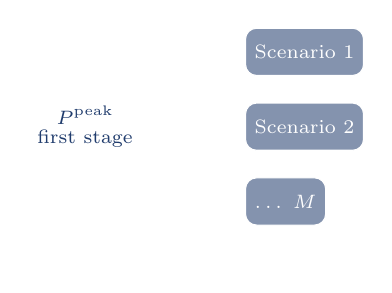
\begin{tikzpicture}[
    every node/.style={font=\scriptsize, text=white},
    trunk/.style={rectangle, draw=white, rounded corners, fill=white,
                  text=lmublue, align=center, minimum height=0.8cm},
    leaf/.style={rectangle, draw=white, rounded corners, fill=lmublue!55,
                 text=white, align=center, minimum height=0.6cm},
    arrow/.style={-{Stealth[scale=1.0]}, white, thick}
]
    \node[trunk] (root) {$P^{\text{peak}}$\\[-1pt]\scriptsize first stage};
    \node[leaf, right=1.3cm of root, yshift=0.95cm]  (s1) {Scenario $1$};
    \node[leaf, right=1.3cm of root]                 (s2) {Scenario $2$};
    \node[leaf, right=1.3cm of root, yshift=-0.95cm] (s3) {$\dots\ M$};
    \draw[arrow] (root) -- (s1);
    \draw[arrow] (root) -- (s2);
    \draw[arrow] (root) -- (s3);
    \node[below=0.15cm of s3, font=\scriptsize] {recourse};
\end{tikzpicture}
\end{column}
\end{columns}
\end{frame}


\end{document}
